\documentclass[11pt]{jsarticle}
\makeatletter
\def\mojiparline#1{
    \newcounter{mpl}
    \setcounter{mpl}{#1}
    \@tempdima=\linewidth
    \advance\@tempdima by-\value{mpl}zw
    \addtocounter{mpl}{-1}
    \divide\@tempdima by \value{mpl}
    \advance\kanjiskip by\@tempdima
    \advance\parindent by\@tempdima
}
\makeatother
\def\linesparpage#1{
    \baselineskip=\textheight
    \divide\baselineskip by #1
}
% 数学の記述 %
\usepackage{amsmath}
\usepackage{amsfonts}
% 左右の余白設定(北大経済の規定)
\usepackage[margin=3cm]{geometry}
% 画像の出力 %
\usepackage[dvipdfm]{graphicx}

\begin{document}
%一行あたり文字数の指定(北大経済の規定)
\mojiparline{35}
%1ページあたり行数の指定(北大経済の規定)
\linesparpage{30}

% abstract
\section*{摘要}
スタッフスケジューリングに関する研究は,Dantzigの高速道路の料金所スタッフに関する論文を皮切りに盛んにおこなわれている.特に数理モデルの開発という点では,鉄道会社や航空会社のスタッフを対象としたクルースケジューリングや,看護師を対象としたナーススケジューリングなど,各業界特有の事情を考慮したモデルが報告されており,現在では非常に多数の研究成果が発表されている.

病院や飲食店のように,勤務形態としてシフト制を採用している職場の多くでは,スタッフがあるシフトを担当するためには,そのシフトに対する担当スキルを所持していることが前提となる.またそのような職場では,未熟なスタッフに対する研修や指導も非常に重要な要素である.特にアルバイトスタッフを主力とした職場では,短期間のうちに研修スタッフが正規スタッフとなり,スタッフのスキルが勤務計画作成の対象期間内で変化するということが度々起こりうる.しかし,それらのことを考慮した数理モデルの開発はこれまでおこなわれてこなかった.そこで本稿では,勤務計画作成の対象期間内において,研修によってスタッフのスキルが変化することを考慮に入れたスタッフスケジューリング問題を扱い,これに対する整数計画モデルを提案する.さらに,実際の現場のデータを用いて数理最適化汎用ソルバーによる計算実験をおこない,提案したモデルの性能評価をおこなった.その結果,通常のコンピュータを用いて約10秒の計算時間で実績を上回る解を求めることができた.実務においては勤務計画の作成に約5 - 7日程度要するため,本稿の提案する手法によって作成の手間を大幅に減らすことができたといえる.

\thispagestyle{empty}
\newpage

% 目次
\tableofcontents
\pagenumbering{roman}
\newpage

\setcounter{page}{1}
\pagenumbering{arabic}
\section{はじめに}
スタッフスケジューリングに関する研究は,Dantzigの高速道路の料金所スタッフに関する論文\cite{bib:dantzig}を皮切りに盛んにおこなわれている.特に数理モデルの開発という点では,鉄道会社や航空会社のスタッフを対象としたクルースケジューリング\cite{bib:air}や,看護師を対象としたナーススケジューリング\cite{bib:nurse_1, bib:nurse_2}など,各業界に特有の事情を考慮したモデルが報告されており,現在では非常に多数の研究成果が発表されている\cite{bib:survey_1, bib:survey_2}.

病院や飲食店のように,勤務形態としてシフト制を採用している職場の多くでは,スタッフがあるシフトを担当するためには当該シフトの担当スキル (以下,単にスキルという) を所持していることが条件となる.アルバイトスタッフを主力とする職場のシフトは,そのシフト内でおこなう作業は単純なものであることが多く,1週間から3週間程度の比較的短期間の職場内教育(以下,研修という)によってスキルを獲得することができ,研修を受けるスタッフにはそのことが期待されている.また,そのような職場では短期間のうちに新規雇用者と離職者が発生するという特徴を持っている.ゆえに,前述のような状況に置かれた現場管理者は職場の安定的な運営のため,未熟なスタッフを指導役のスタッフとともにシフトへ参加させ,日々の業務をおこないながら同時に研修もおこなう (これは一般にOJT (On the Job Training) 方式と呼ばれる\cite[pp.27-28]{bib:ojt})ということを考慮に入れながら勤務計画を作成している.言い換えれば,各スタッフのスキルを変化させることを念頭に置いて勤務計画を作成している.

これまでにスキルと研修を扱ったスタッフスケジューリング研究としては,\cite{bib:senkou_Off, bib:senkou2, bib:senkou_Israel, bib:senkou1}が挙げられる.LiangとBuclatin\cite{bib:senkou_Off}は,Off-JT (Off the Job Training) 方式による研修,すなわち研修の場と日々の業務の場が異なることを前提としてモデルを作成しており,研修スタッフにどのようなスキルを身に着けさせるべきか,ということを主な問題としている.Sinuany-SternとTeomi\cite{bib:senkou_Israel}は,研修を毎月スタッフ全員が複数回入らなければならない (特殊な) シフトとして扱っている.すなわち,研修はそれを終えてはじめてスキルを獲得することができるといった性質を持たず,スキルと研修が直接結びついていないモデルとなっている.Yuuraら\cite{bib:senkou1}は,放射線技師を対象にOJT方式での研修が想定されているものの,研修期間について (半ば暗黙に) 長期であることが仮定されており,勤務計画作成の対象期間内での各スタッフのスキルの有無は,既にモデル外で決定されているものとして扱われている.つまり,勤務計画の対象期間内では正規スタッフと研修スタッフが明確に区別されて扱われている.MiyamotoとHidaka\cite{bib:senkou2}は\cite{bib:senkou1}を改良したモデルを提案しているが,スキルや研修といったものの扱いは同様である.ゆえに,アルバイトスタッフを主力とする職場のように短期間で研修スタッフから正規スタッフへと変化しうる状況下では,これらのモデルを適用することは困難である.

そこで本稿では,勤務計画作成の対象期間内に研修スタッフが (研修によって) 必要なスキルを獲得し,正規の業務も担当可能になることを考慮に入れたスタッフスケジューリング問題を扱い,これに対する整数計画モデルを提案する.さらに,実際の現場のデータを用いて計算実験をおこない,モデルの性能を検証する.その結果,実績を上回る勤務計画を作成することができた.

本稿の構成は以下の通りである.第2章では本研究で取り扱う整数計画モデルを提示する.第3章では,実際の現場のデータを用いて計算実験をおこなう.また,計算実験による勤務計画と,実際の現場で用いられた手作業による勤務計画を比較・分析し,作成したモデルの性能を検証する.第4章ではまとめをおこなう.
\newpage

\section{最適化モデル}
\subsection{諸定義}
スタッフの集合を$A$とする.勤務計画を考える日付の集合を$N = \{ 1, 2, ..., n_{\ell} \}$とする.シフトの集合を$S$で表す.各シフト$s \in S$は,それぞれそのシフトの開始時刻を情報として持ち,それを$s_{time}$で表す.2つのシフト$s, \ s^{\prime} \in S$があるとき,$s_{time} \geq s_{time}^{\prime}$であればシフト$s$のほうがシフト$s^{\prime}$より開始時刻が遅いことを表す.

各スタッフ$a \in A$の月当たりの契約勤務回数を$O_a$で表す.$j \ (\in N)$日のシフト$s \in S$に割り当てなければならない最低限の人数を$\ell_{js}$で表し,上限人数を$u_{js}$で表す.$\delta_{as}$を,勤務計画作成前の段階においてスタッフ$a \in A$がシフト$s \in S$を独力で担当できれば1,そうでなければ0をとるパラメータとし,スタッフの休暇希望申請に関して$r_{aj}$を,スタッフ$a \in A$が$j \ (\in N)$日に休暇を希望するとき1,それ以外は0であるようなパラメータとする.$h_{aj}$を,スタッフ$a \in A$が$j \ (\in N)$日にシフト$s^{\prime} \in S$を希望するとき$h_{aj} = s^{\prime}$を取るようなパラメータとし,そのシフト$s^{\prime}$より開始時刻が早いシフト集合を$S_{imp}(a, j) = \{s \in S \ |s_{time} < s_{time}^{\prime} \}$で表す.

$\theta_{as}$を,スタッフ$a \in A$についてシフト$s \in S$での研修を計画しているとき1,そうでなければ0を取るパラメータとする.ただし研修計画は,現場管理者の経営判断によってあらかじめ決定されているものとする.$\xi_{as}$を,スタッフ$a \in A$がシフト$s \in S$の指導スキルを所持しているとき1,そうでなければ0をとるパラメータとする.ただし,$\xi_{as} \leq \delta_{as}$である.研修が必要なスタッフ$a \in A$が受けなければならない研修シフトの回数を$t_{as}$とし,$c_{as} \ (0 \leq c_{as} \leq t_{as})$を,スタッフ$a \in A$が勤務計画作成前の段階において,研修スタッフとして既にこなしたシフト$s \in S$の回数とする (つまり,あと$t_{as} - c_{as}$回研修を受けることでスタッフ$a$はシフト$s$を独力で担当可能となる).ただし,研修の必要がないスタッフについては$t_{as} = c_{as} = 0$と定める.スタッフ$a \in A$が研修を予定していないシフト集合を$S_{ban}(a) = \{ s \in S \ | \theta_{as} = 0 \}$で表す.

決定変数は以下の通りである.$\lambda_{ajs}$をスタッフ$a \in A$の$j \ (\in N)$日におけるシフト$s \in S$のスキル習熟度とし,スタッフ$a$の$j$日のシフト$s$について研修を必要としない状態,すなわちシフト$s$を独力で担当できる状態のとき1であり,それ以外は0であるような0-1変数とする.$x_{ajs}$をスタッフ$a \in A$が$j \ (\in N)$日のシフト$s \in S$にシフトを独力で担当するとき1,それ以外は0であるような0-1変数とし,$y_{ajs}$をスタッフ$a \in A$が$j \ (\in N)$日のシフト$s \in S$を研修シフトとして担当するとき1,それ以外は0であるような0-1変数とする.その他に,$d_{as}, e_{ajs}, \check{f_a}, \hat{f_a} $を制約式 (\ref{t_3}), (\ref{t_5}), (\ref{i_3}) のペナルティ変数として用意するが,詳細については2.2節で説明する.

\vspace{\baselineskip}
\subsection{制約式}
本稿のスケジューリング問題において満たすべき制約条件式を説明する.ここで(\ref{st_1})~(\ref{st_3})式はシフトを担当するための条件とスキルに関する制約であり,(\ref{t_1})~(\ref{t_5}) 式は研修に関する制約である.また,(\ref{i_1})~(\ref{i_5}) 式はスタッフスケジューリングにおける基本的な制約である.
\begin{equation}
x_{ajs} \leq \lambda_{ajs} \ (\forall a \in A , \ \forall j \in N, \ \forall s \in S)
\label{st_1}
\end{equation}
\begin{equation}
\delta_{as} \leq \lambda_{ajs} \ (\forall a \in A, \ \forall j \in N, \ \forall s \in S)
\label{st_2}
\end{equation}
\begin{equation}
\delta_{as} = 0 \Rightarrow \ \lambda_{ajs} \leq \theta_{as} \ (\forall a \in A, \ \forall j \in N, \ \forall s \in S)
\label{st_3}
\end{equation}

(\ref{st_1}) 式は,スタッフ$a \in A$が$j \ (\in N)$日までにシフト$s \in S$のスキルを保持していない ($\lambda_{ajs} = 0$) とき,スタッフ$a$は$j$日にシフト$s$を独力で担当しない ($x_{ajs} = 0$) ことを表す.一方,スタッフ$a$が$j$日までにシフト$s$のスキルを保持している ($\lambda_{ajs} = 1$) とき,$x_{ajs}$は0と1のどちらもとりうる. (\ref{st_2}) 式は,勤務計画作成前の段階において,スタッフ$a \in A$がシフト$s \in S$のスキルを所持している ($\delta_{as} = 1$) とき,スタッフ$a$は任意の$j \ (\in N)$日についてシフト$s$を独力で担当可能であるから,勤務計画作成の対象期間内においては研修が必要なく,独力でシフト$s$を担当できる状態 ($\lambda_{ajs} = 1$) であることを表す. (\ref{st_3}) 式は,勤務計画作成前の段階でスタッフ$a \in A$にシフト$s \in S$を担当するスキルがなく ($\delta_{as} = 0$),かつ当該シフトの研修も計画されていない ($\theta_{as} = 0$) のであれば,スタッフ$a$はシフト$s$を独力で担当することができず研修が必要な状態 ($\lambda_{ajs} = 0$) のままであるということを表したものである.
\begin{equation}
\sum_{s \in S_{ban}(a)} y_{ajs} \leq 0 \ (\forall a \in A, \ \forall j \in N)
\label{t_1}
\end{equation}
\begin{equation}
\sum_{a \in A} y_{ajs} \leq 1 \ (\forall j \in N, \ \forall s \in S)
\label{t_2}
\end{equation}

(\ref{t_1}) 式は,スタッフ$a \in A$が,定められた研修シフト以外のシフトに研修として入ることを禁止するものである. (\ref{t_2}) 式は,同日の1つのシフトについて研修スタッフは2人以上入ることはできず,高々1人までという規則を表したものである.
\begin{equation}
t_{as} - d_{as} \leq c_{as} + \sum_{j \in N} y_{ajs} \leq t_{as} \ (\forall a \in A, \ \forall s \in S)
\label{t_3}
\end{equation}
\begin{eqnarray}
(t_{as} - c_{as}) \ \lambda_{ajs} \leq \sum_{k = 1}^{j} y_{aks} \ (\forall a \in A, \ \forall j \in N, \ \forall s \in S)
\label{t_4}
\end{eqnarray}

(\ref{t_3}) 式は,シフト$s \in S$について研修が必要なスタッフ$a \in A$は,研修シフトを勤務計画作成の対象期間内に定められた回数こなさなければならないということを表したものである.ただし,スタッフや職場の事情によって規定の回数である$t_{as}$をこなすことが難しい場合がある.ゆえにペナルティ変数である$d_{as}$を設定することで,対象期間内にできるだけ規定回数へ近づけるように要請する制約式 (このような制約を考慮制約という) としている.また,研修を終えた後は当該シフトについて,もはや研修スタッフではなく普通のスタッフとして独力でシフトを担当することが期待されているため,研修回数には下限だけではなく上限も設けている.一方 (\ref{t_4}) 式では,必要な回数($t_{as} - c_{as}$)分の研修を受けていない間は,スキルを保持していない ($\lambda_{ajs} = 0$) 状態のままであることを表す.
\begin{equation}
\theta_{as} y_{ajs} \leq \sum_{i \in A} \xi_{is} x_{ijs} + e_{ajs} \ (\forall a \in A, \ \forall j \in N, \ \forall s \in S)
\label{t_5}
\end{equation}

(\ref{t_5}) 式は,スタッフ$a \in A$が研修でシフト$s \in S$に入るときは,なるべく指導スキルを所持しているスタッフ$i \in A$が同時に教育係としてシフトに入らなければならないということを表したものである.なお,$e_{ajs}$はこの制約に対するペナルティ変数である.
\begin{equation}
\sum_{s \in S} \ (x_{ajs} + y_{ajs}) \leq 1 \ (\forall a \in A, \ \forall j \in N)
\label{i_1}
\end{equation}
\begin{equation}
\ell_{js} \leq \sum_{a \in A} x_{ajs} \leq u_{js} \ (\forall j \in N, \ \forall s \in S)
\label{i_2}
\end{equation}
\begin{equation}
O_a - \check{f_a} \leq \sum_{j \in N}\sum_{s \in S} \ (x_{ajs} + y_{ajs}) \leq O_a + \hat{f_a} \ (\forall a \in A)
\label{i_3}
\end{equation}
(\ref{i_1}) 式は,各日において1人のスタッフが研修シフトも含めて複数のシフトを兼任することはできないという規則を表したものである. (\ref{i_2}) 式は,各日の個別のシフトにおいて割り当てなければならない人数の上下限制約である. (\ref{i_3}) 式は,各スタッフの,契約時に定められた月当たりの契約勤務回数をできるだけ守るよう要請することを表したものである.この契約勤務回数を大幅に違反しても問題はないが,この回数はスタッフの意向が反映されたものであるから,この制約はできるだけ満たすのが望ましい.なお,$ \check{f_a}, \  \hat{f_a} $はペナルティ変数であることに注意する.
\begin{equation}
\sum_{j \in N}\sum_{s \in S}r_{aj} (x_{ajs} + y_{ajs}) \leq 0 \ (\forall a \in A)
\label{i_4}
\end{equation}
\begin{equation}
h_{aj} = s^{\prime} \Rightarrow \sum_{s \in S_{imp}(a, j)} (x_{ajs} + y_{ajs}) \leq 0 \ (\forall a \in A, \ \forall j \in N)
\label{i_5}
\end{equation}

(\ref{i_4}) 式はスタッフの休暇希望申請に関する制約であり,スタッフ$a \in A$が$j \ (\in N)$日に休暇を希望するときそのスタッフは$j$日のどのシフト$s \in S$にも割り当てられないことを表したものである. (\ref{i_5}) 式は,スタッフ$a \in A$が$j \ (\in N)$日に$s^{\prime} \in S$というシフト希望したとき,そのシフトより早い時刻から開始するシフトは割り当てないということを表したものである.

\vspace{\baselineskip}
\subsection{整数計画問題としての定式化}
職場内教育を考慮したスタッフスケジューリングの整数計画問題は次のように与えられる.
\begin{align}
    \min
    &
    \ \ w_1 \sum_{a \in A}\sum_{j \in N}\sum_{s \in S}(1 - \lambda_{ajs}) + w_2 \sum_{a \in A}\sum_{s \in S} d_{as} + w_3 \sum_{a \in A}\sum_{j \in N}\sum_{s \in S} e_{ajs} \nonumber
    & \\ &
    + w_4 \sum_{a \in A}(\check{f_{a}} + \hat{f_{a}})
    \label{optimize}
    \\
    \mathrm{s. \ t. }
    &
    \ \ (\ref{st_1}) - (\ref{i_5})
    \nonumber
\end{align}
ここで (\ref{optimize}) 式の第1項は,$\lambda_{ajs}$の値をできるだけ早い時期に1にすること,言い換えれば,研修の早期完了を目的とするものである.一方,第2, 3, 4項はそれぞれ (\ref{t_3}), (\ref{t_5}), (\ref{i_3}) 式の制約に対するペナルティ (違反度合) を最小にすることを目的としている.また,$w_1, ..., w_4$を各ペナルティに対する非負実数の重みとする.特に条件を満たしていてほしい制約について,それに対応する重み$w_i$に大きな値を設定することでその制約をより厳しく守るスケジュールを作成することができる.

\newpage
\section{計算実験と考察}
\subsection{計算環境とデータ}
提案したモデルの評価をするために,筆者のアルバイト先である飲食店を対象に,2019年6月度における実際の現場のデータを用いて計算実験をおこなった.なお,計算にはソフトウェアにPython 3.7.1の付属パッケージであるPuLP 1.6.5 \cite{bib:pulp}を用いた.また,計算環境はCPUがIntel Core M-5Y10c 0.80GHz (2コア) ,メモリが4GBである.
%表1
\begin{table}[b]
  \begin{center}
    \caption{各シフトの勤務時間帯}
    \begin{tabular}{cl}
      \hline \hline
      シフト名 & 勤務時間帯 \\ \hline
      1 & 15:00-19:30 \\
      2 & 16:45-19:30 \\
      3 & 17:00-19:30 \\
      4 & 15:00-19:30 \\
      5 & 15:30-19:30 \\
      6 & 17:30-19:30 \\
      7 & 17:30-19:30 \\
      21 & 10:00-14:30 \\
      22 & 10:30-14:30 \\
      23 & 12:00-14:30 \\
      24 & 10:00-14:30 \\ \hline \hline
    \end{tabular}
    \label{tab:shift_time}
  \end{center}
\end{table}

%表2
\begin{table}[htb]
  \begin{center}
    \caption{シフト構成と上下限人数}
    \begin{tabular}{clllllllllll}
      \hline \hline
      シフト構成 & 1 & 2 & 3 & 4 & 5 & 6 & 7 & 21 & 22 & 23 & 24 \\ \hline
        A & 0 & 1 & 1 & 0 & 1 & 1 & 1 & 0 & 0 & 0 & 0 \\
        B & 1 & 0 & 1 & 1 & 1 & 1 & 1 & 0 & 0 & 0 & 0 \\
        C & 0 & 1 & 1 & 1 & 1 & 1 & 1 & 0 & 0 & 0 & 0 \\
        D & 0 & 0 & 0 & 0 & 0 & 0 & 0 & 1 & 1 & 1 & 1 \\ \hline \hline
    \end{tabular}
    \label{tab:shift_construct}
  \end{center}
\end{table}

%表3
\begin{table}[htb]
	\begin{center}
    \caption{各スタッフの月当たりの契約勤務回数と担当可能なシフト}
    \begin{tabular}{ccl}
      \hline \hline
      スタッフ & 契約勤務回数 (回/月) & 担当可能なシフト \\ \hline
      1* & 10 & 1, 2, 3, 4, 5, 6, 21, 22, 23 \\
      2* & 10 & 1, 2, 3, 21 \\
      3* & 10 & 4, 5, 6, 22, 23 \\
      4* & 10 & 1, 2, 3, 7, 21, 24 \\
      5* & 10 & 4, 5, 6, 22, 23 \\
      6* & 10 & 1, 2, 3, 5, 6, 21, 22, 23 \\
      7* & 10 & 1, 2, 3, 5, 6, 21 \\
      8* & 10 & 1, 2, 3, 21 \\
      9* & 5 & 7, 24 \\
      10* & 5 & 4, 5, 6, 22, 23 \\
      11 & 10 & 4, 5, 6, 7, 22, 23, 24 \\
      12 & 10 & (5 - 5), 6, 22, 23 \\
      13 & 15 & 5, 6, 22, 23 \\
      14 & 15 & 1, 2, 3, 21 \\
      15 & 15 & (7 - 5), (24 - 2) \\ \hline \hline
    \end{tabular}
    \label{tab:staff_skill_contract}
  \end{center}
\end{table}
問題の規模は,$|A| = 15, \ |N| = 25, \ |S| = 11$である.各シフトの勤務時間帯は表\ref{tab:shift_time}のとおりである.シフト1から7は平日の業務に必要なシフトであり,シフト21から24は土曜日の業務に必要なシフトである.表\ref{tab:shift_construct}はシフト構成を表したものである.対象とした飲食店では,通常シフト2, 3, 5, 6, 7を組み合わせたシフト構成を取っている (これを構成Aと呼ぶ).他にも,シフト2の代わりにシフト1とシフト4が追加される構成Bや,構成Aにシフト4が追加される構成C,土曜日のシフトであるシフト21, 22, 23, 24が必要となる構成Dがある (表\ref{tab:shift_construct} 参照). また,表\ref{tab:staff_skill_contract}は各スタッフの月当たりの契約勤務回数と担当可能なシフトを列挙した表である.なお,担当可能なシフト項目においてかっこ書きがなされたものは,当該スタッフは未だそのシフトの担当スキルを獲得していないものの,勤務計画作成の対象期間内に研修シフトが予定されていることを表し,ハイフンの後ろは研修回数($t_{as} - c_{as}$)を表す.また,今回の分析では,入社後半年以上をもって指導スキルは自動的に獲得するものとして扱った.アスタリスクがついているスタッフは,自身の担当可能なシフトについてはすべて指導スキルを有しており,アスタリスクがついていないスタッフは,担当可能なシフトであっても当該シフトの指導スキルは有さない.図\ref{fig:shift_preference}は各スタッフの勤務計画作成の対象期間における勤務希望を表したものである.ただし,10はその日に休暇希望申請を出していることを表し,それ以外の数字については,その番号のシフトと同じかそれより開始時刻が遅いシフトについては勤務可能であることを表す.また各日のシフト構成はあらかじめ定められており,図\ref{fig:shift_preference}の最下行にまとめられている.重みは研修の早期完了と月当たりの契約勤務回数を重視し,$w_1 = 5, \ w_2 = 5, \ w_3 = 1, \ w_4 = 3$と設定した.

%図1(希望表)
\begin{figure}
  \begin{center}
    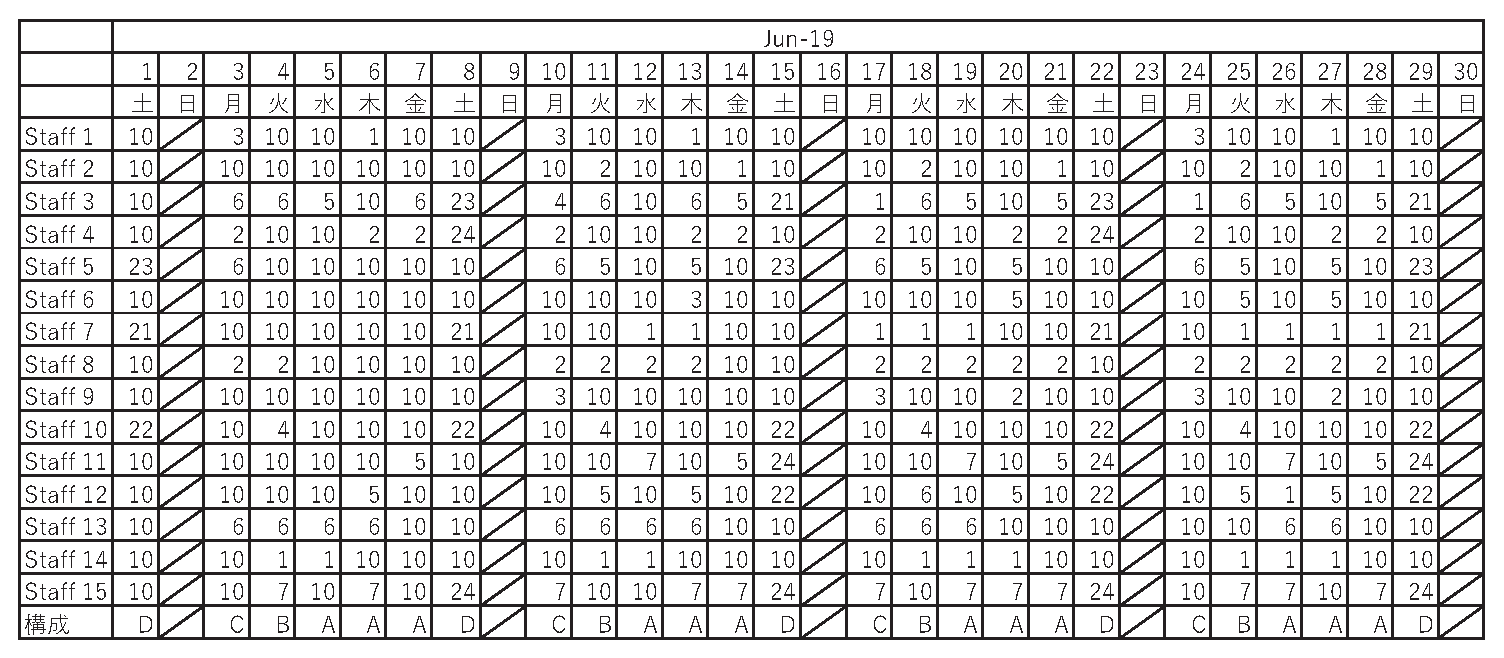
\includegraphics[width = 13.2cm]{figs/june_preference.eps}
  \end{center}
  \caption{各スタッフの勤務希望}
  \label{fig:shift_preference}
\end{figure}

2.3節のモデルに従って実験をおこなったところ,休暇希望申請をすべて満たし,かつシフトの下限制約を満たす解は存在しないことがわかった.このような理由として,対象の飲食店固有の事情であるが,スタッフの休暇希望申請については「本当はシフトに入ることは可能であるものの,積極的にシフトに入りたいというわけではない」という意味での申請が頻繁にあり,必要以上に休暇希望申請が出ていたことが考えられる.そのような場合,実務においては休暇希望申請がどのような理由でなされたものかについて判別がつかないことから,一度各スタッフの休暇希望申請をすべて満たすようなスケジュールを作成し,担当者が不足するシフトは不足欄にまとめて掲示される (図\ref{fig:operation}は実際の現場で用いられた手作業による勤務計画であるが,担当者が不足しているシフトは多数存在することが確認できる).その後担当者が不足するシフトについては,それが実行される当日までに現場管理者の方から,当該シフトのスキルを持つ各スタッフへ,その日に当該シフトが担当可能かどうか確認するための連絡がなされる.それに応じて「本当はシフトに入ることは可能であるものの,積極的にシフトに入りたいというわけではない」という意味で休暇希望申請を出したスタッフが,担当可能である旨を現場管理者に伝えることで当該シフトの担当者が決定される.前述のとおり,この「積極的にシフトに入りたいというわけではない」という意味での休暇希望申請は頻繁にあるため,今回の事例においては,シフトの下限制約を緩めてもさほど大きな影響はないと考えられる.

%表4
\begin{table}[htb]
  \begin{center}
    \caption{各シフトの担当スキルを持つ人数と重み}
    \label{tab:shift_can_num}
    \begin{tabular}{ccc}
      \hline \hline
      シフト & 人数 & $w_{5,s}$ \\ \hline
      1 & 7 & 13 \\
      2 & 7 & 13 \\
      3 & 7 & 13 \\
      4 & 6 & 14 \\
      5 & 8 & 12 \\
      6 & 9 & 11\\
      7 & 3 & 17\\
      21& 7 & 13 \\
      22 & 8 & 12 \\
      23 & 8 & 12 \\
      24 & 3 & 17\\ \hline \hline
    \end{tabular}
  \end{center}
\end{table}
よって以下では,第2章で示したモデルの (\ref{i_2}) 式に対してペナルティ変数$g_{js}$を導入し,(\ref{i_2_a}) 式のように変更する.
\begin{equation}
\ell_{js} - g_{js} \leq \sum_{a \in A} x_{ajs} \leq u_{js} \ (\forall j \in N, \ \forall s \in S)
\label{i_2_a}
\end{equation}
言うまでもないことであるが,シフトの下限制約は極力満たす方が望ましいため,非負実数の重み$w_{5,s}$を設定したうえで (\ref{optimize}) 式に第5項として $\displaystyle \sum_{j \in N} \sum_{s \in S} w_{5,s} \ g_{js} $を追加する.また,前述の実務での対応状況から,担当者が不足するシフトはなるべく担当スキルを持つスタッフが多いシフトの方が望ましい.これは,一般に連絡可能なスタッフが増えれば増えるほど,当該シフトを担当することができると答えるスタッフに当たる可能性が高くなるためである.このような事情から$w_{5,s}$には,担当スキルを持つスタッフが多いシフト$s \in S$には小さい値を,担当スキルを持つスタッフが少ないシフト$s \in S$には大きい値を設定する.表\ref{tab:shift_can_num}に各シフトの担当スキルを所持するスタッフの数と,それを基に決定した$w_{5,s}$の値を示す.また,その他の重みについては前述のとおり$w_1 = 5, \ w_2 = 5, \ w_3 = 1, \ w_4 = 3$とする.$w_{5,s}$を$w_1, \ w_2, \ w_3, \ w_4$より大きな値とする理由は,シフトの下限制約を満たすことは日々の業務が滞りなくおこなわれるためにも不可欠だからである.以上の変更を加えて再度実験をおこなった.

%図2(最適解図)
\begin{figure}
  \begin{center}
    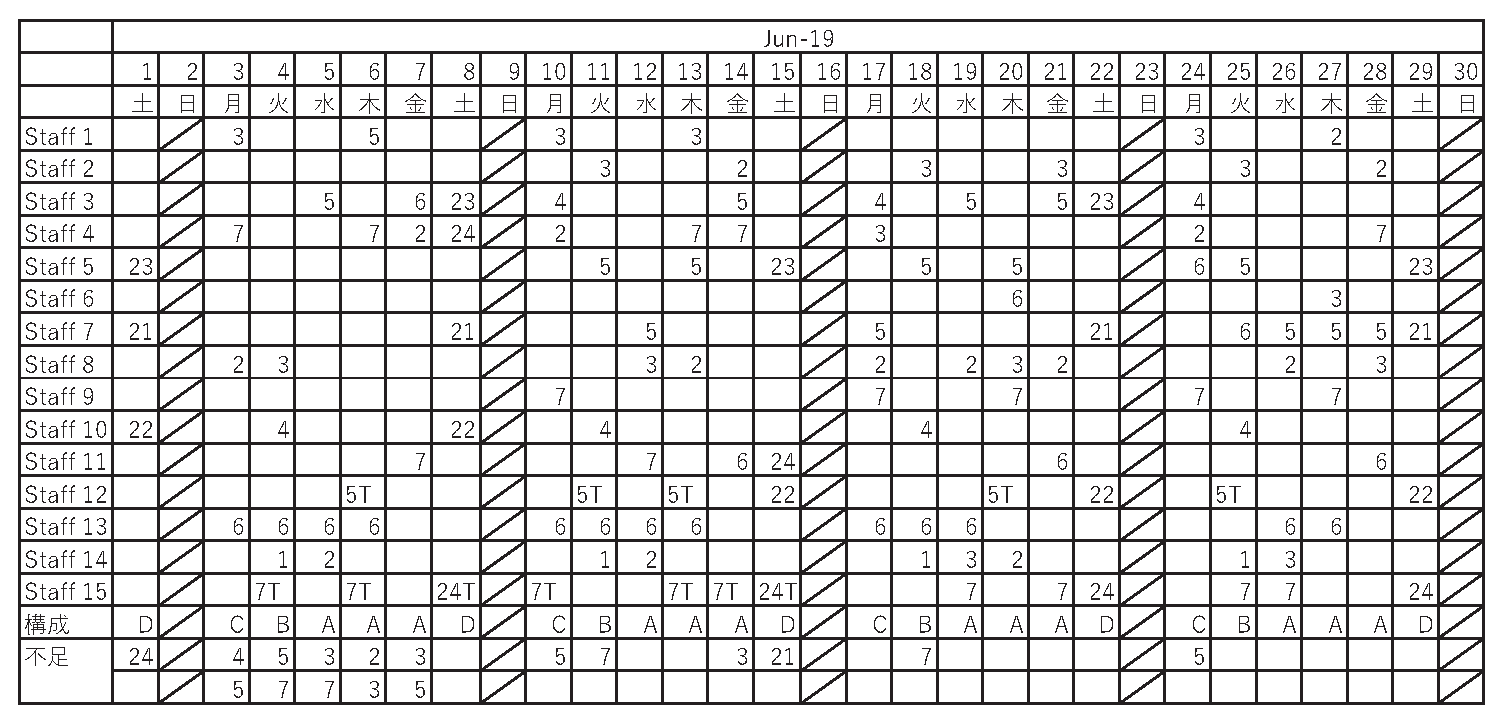
\includegraphics[width = 13.2cm]{figs/june_optimal.eps}
  \end{center}
  \caption{計算実験による勤務計画 (Tは研修シフトであることを表す)}
  \label{fig:optimal}
\end{figure}
%図3(運用図)
\begin{figure}
  \begin{center}
    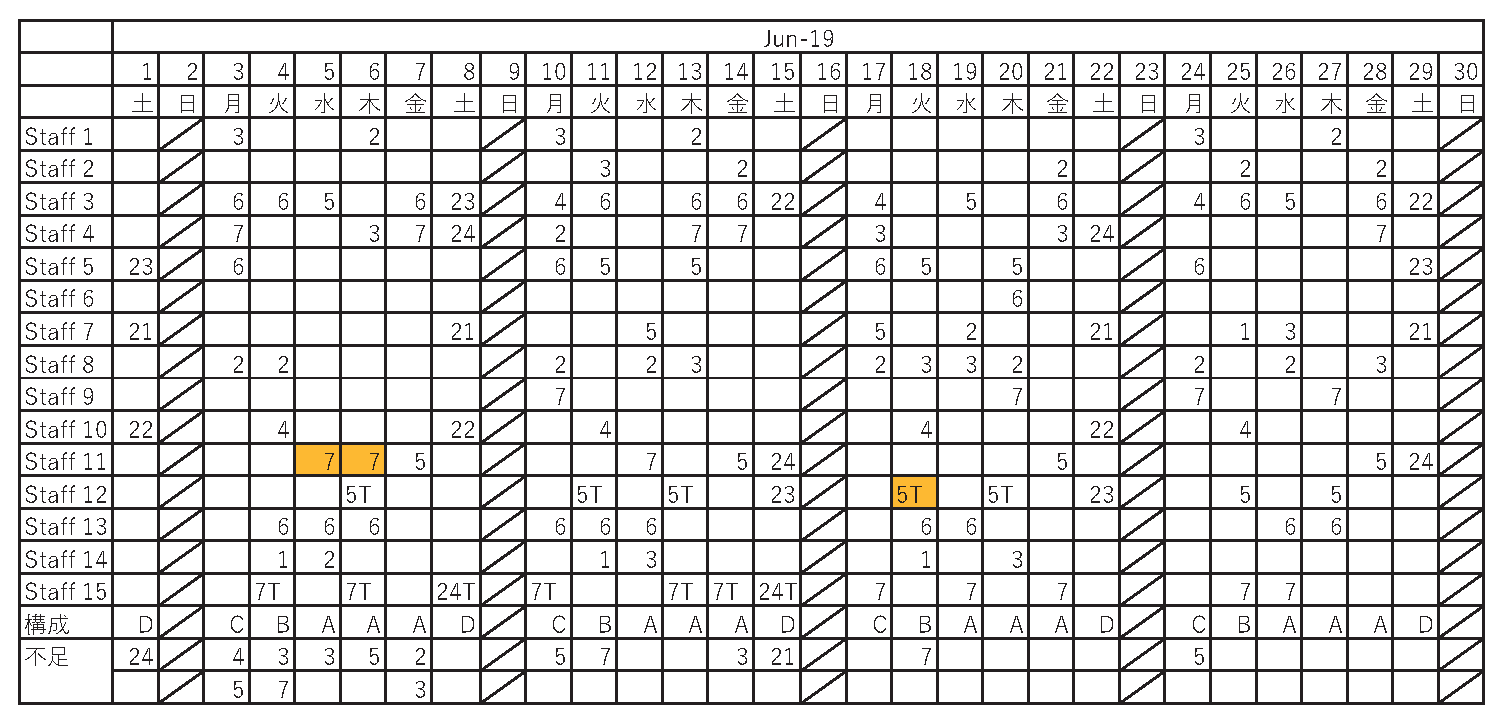
\includegraphics[width = 13.2cm]{figs/june_operation.eps}
  \end{center}
  \caption{手作業による勤務計画 (Tは研修シフトであることを表す)}
  \label{fig:operation}
\end{figure}

\vspace{\baselineskip}
\subsection{結果と考察}
3.1節に従って変更された整数計画問題は変数が16,970個,制約式は24,971本であり,求解までに要した時間は10.3074秒であった.図\ref{fig:optimal}は3.1節の計算結果により得られた勤務計画 (以下,計算実験による勤務計画という) であり,図\ref{fig:operation}は,前述のとおり実際の現場で用いられた手作業による勤務計画 (以下,手作業による勤務計画という) である.なお,図の下部の不足欄には担当者が不足するシフトがまとめて表示されている.また図\ref{fig:operation}の一部には,ミスにより休暇希望申請を出しているのにも関わらずシフトが割り当てられている部分 (スタッフ11は,5, 6日に休暇希望申請を出しているが,シフト7が割り当てられている) や,時間の希望が考慮されていない部分 (スタッフ12は,18日に17:30以降の勤務を希望しているが,15:30開始のシフト5が割り当てられている) があるため,そのような箇所を着色している.

本節では,この2つの勤務計画を (a) 担当者が不足するシフトはどのような性質をもっているか (b) 研修の早期完了という目標は達成されているか (c) 研修は適切な教育スタッフの下でおこなわれているか (d) 各スタッフの勤務回数は月当たりの契約勤務回数に沿っているかという4つの点から比較をおこなう.

\vspace{\baselineskip}
\subsubsection*{(a) 担当者が不足するシフトの性質}
担当者不在のシフトについて,計算実験による勤務計画と手作業による勤務計画とでは,不足するシフト数は (ミス部分を除くと) すべての日にちで一致するなど大方同様の結果となった.また計算実験による勤務計画では,4日についてはシフト3のかわりにシフト5を,7日についてはシフト2のかわりにシフト5を担当者不在としているが,それぞれのシフトの担当人数については表\ref{tab:shift_can_num}の通りほぼ同様であることから,さほど大きな変化はない.しかし6日について着目すると,計算実験による勤務計画はスタッフ4をシフト7に割り当てており,担当スキルをもつスタッフ数がより少ないシフトを優先している.さらに,計算実験による勤務計画ではスタッフ1がシフト5に割り当てられているが,手作業による勤務計画ではスタッフ1がシフト2に割り当てられており,2つの勤務計画で相違があった.この理由としては,計算実験による勤務計画では研修の早期完了という目標のため,指導スキルを有するスタッフの確保が優先されたと考えられる.なお,手作業による勤務計画ではシフト5に研修スタッフが割り当てられているにも関わらず,教育スタッフが割り当てられていないことに注意する.

\vspace{\baselineskip}
\subsubsection*{(b) 研修の早期完了}
研修が予定されているスタッフは12と15であり,両者の勤務計画を比較する.計算実験による勤務計画では,18日についてスタッフ12はシフト6以降の時間帯を希望しているのに対し,シフト5の研修を割り当ててしまうというミスがあるものの,どちらの勤務計画も両者の休暇希望申請を考慮しながら比較的短期間で規定の回数の研修をこなすことができていると考えられる.

\vspace{\baselineskip}
\subsubsection*{(c) 適切な教育スタッフの下での研修}
前述のとおり今回の分析では,指導スキルは入社後半年以上をもって自動的に獲得するものとして扱った.2019年6月度においてはスタッフ1から10の,それぞれの担当可能シフトについては指導スキルを有している状態であり,スタッフ11から15は指導スキルを有していない状態であった.

研修シフトについて着目すると,計算実験による勤務計画ではスタッフ1, 5が,スタッフ12の研修シフト5の教育スタッフとして割り当てられている.また,手作業による勤務計画では主にスタッフ5が教育スタッフとして割り当てられているため,どちらも適切な教育スタッフがついているといえる.一方スタッフ15の研修については,2つの勤務計画はどちらも,主にスタッフ4が教育スタッフとして割り当てられている.しかし6日については,スタッフ4がシフト7を担当することができ,かつスタッフ11が休暇を希望している状態であるにも関わらず,手作業による勤務計画では,スタッフ11がシフト7へ割り当てられている.6日は,計算実験による勤務計画のようにスタッフ1にシフト5を,スタッフ4にシフト7を割り当て,シフト2, 3は不足欄へと入れることで,より望ましい勤務計画を作成できる可能性がある.

\vspace{\baselineskip}
%表5
\begin{table}[htb]
  \begin{center}
    \caption{勤務回数の比較 (回/月) }
    \begin{tabular}{cccc}
      \hline \hline
      スタッフ名 & 図2の勤務回数 & 図3の勤務回数 & 契約勤務回数 \\ \hline
      1 & 6 & 6 & 10 \\
      2 & 6 & 5 & 10 \\
      3 & 10 & 18 & 10 \\
      4 & 10 & 11 & 10 \\
      5 & 9 & 10 & 10 \\
      6 & 2 & 1 & 10 \\
      7 & 10 & 9 & 10 \\
      8 & 10 & 12 & 10 \\
      9 & 5 & 5 & 5 \\
      10 & 6 & 7 & 5 \\
      11 & 6 & 9 & 10 \\
      12 & 8 & 9 & 10 \\
      13 & 13 & 10 & 15 \\
      14 & 9 & 6 & 15 \\
      15 & 13 & 12 & 15 \\ \hline \hline
    \end{tabular}
    \label{tab:compare}
  \end{center}
\end{table}
%表6
\begin{table}[htb]
  \begin{center}
    \caption{契約勤務回数との差の平均}
    \begin{tabular}{ccc}
      \hline \hline
      & 計算実験による勤務計画 (回) & 手作業による勤務計画 (回) \\ \hline
      平均値 & 2.2667 & 3.4000 \\ \hline \hline
    \end{tabular}
    \label{tab:mean_stdev}
  \end{center}
\end{table}
\subsubsection*{(d) 各スタッフの勤務回数と月当たりの契約勤務回数}
スタッフの月当たりの契約勤務回数は表\ref{tab:compare}の通りであるが,実際の勤務回数は契約勤務回数に近い (すなわち,契約勤務回数と勤務計画による勤務回数の差の絶対値が小さい) 方が望ましい.ここでスタッフ3に着目してみると,契約勤務回数は10回であるにも関わらず,手作業による勤務計画では18回の勤務を要請している.また,スタッフ13は契約勤務回数が15回であるが,手作業による勤務計画では10回しか割り当てられることがなかった.しかし,計算実験による勤務計画ではスタッフ3の勤務回数は10回となり,スタッフ13の勤務回数は13回にまで増えている.実際,契約勤務回数と各勤務計画による勤務回数の差の平均値は,表\ref{tab:mean_stdev}のとおりであった.手作業による勤務計画は契約勤務回数との差が平均3.4回であったが,計算実験による勤務計画は平均2.3回程度であり,計算実験による勤務計画は手作業による勤務計画と比べて契約勤務回数と勤務回数の差がより小さくなっている.ゆえに計算実験による勤務計画は,各スタッフの希望をより反映している勤務計画であるといえる.

\vspace{\baselineskip}
以上の4つの点で比較すると,計算実験による勤務計画は手作業による勤務計画よりも良い結果を示しているといえる.
\newpage

\section{まとめ}
本稿では,職場内教育 (研修) によってスタッフのスキルが変化することを考慮に入れた勤務計画作成問題を考え,これに対する整数計画モデルを構築した.さらに,実際の現場のデータを用いて数理最適化汎用ソルバーによる計算実験をおこなった.その結果,通常のコンピュータを用いて約10秒の計算時間で実績を上回る解を求めることができた.特に,実務においては勤務計画の作成に約5 - 7日程度要するため,本稿の提案する手法によって作成の手間を大幅に減らすことができたといえる.その他具体的に改善された点としては,より適切なスタッフの下での研修を設定ができたことや,実際の勤務回数と月当たりの契約勤務回数との差異を小さくできたことが挙げられる.一方,担当者が不足するシフトや研修の早期完了といった点では,手作業による勤務計画とほぼ同等であるものが見られた.これは,実際の現場のデータではスタッフの休暇希望申請とシフトの下限制約を同時に満たす解は存在せず実行不能となったことから,そもそも解の候補が少なかったことに起因すると考えられる.

実行不能となったのは対象の飲食店固有の事情で,休暇希望申請に「本当はシフトに入ることは可能であるものの,積極的にシフトに入りたいというわけではない」という性質を帯びたものが多く含まれているためである.しかし,各スタッフの休暇希望申請に関する精緻なデータを入手することが困難であったため,実験においても休暇希望申請とシフトの下限制約を同時に満たす解を見つけることを断念せざるを得なかった.スタッフの休暇希望申請のうち「確実に出勤不可能である」ものと「積極的に勤務を希望するわけではない」ものの区別がつく場合は,前者を絶対制約,後者を考慮制約として扱うことで,より実情に合ったモデル化が可能である.さらにそれだけではなく,このことが実現可能であれば,実務でおこなわれていた担当者不足の際の対応を減らすことも期待できる.さらなる勤務計画作成のためには,正確なモデル作成だけでなく現場のデータの取り方についても考慮する余地があり,より総合的な検討が必要である.

また本稿の勤務計画の作成方法では,その作成の際に入力しなければならない項目が多数あり手間がかかる.ゆえに,本稿の方法を実際に現場へ適用することを考えるときには,入力が容易でわかりやすいインターフェイスの開発が必須である.

さらに質の高い勤務計画の作成のためには以上の2点の解決が不可欠であり,これらは今後の課題である.

\section*{謝辞}
本稿の作成にあたって多数の御指導・御助言を頂きました石井利昌教授に心より感謝申し上げます.また,研究を進めるにあたって多数の御指摘をくださったアルバイト先の店長様,石井ゼミの皆さまに心より感謝申し上げます.

\begin{thebibliography}{99}
  \bibitem{bib:air}
    J. P. Arabeyre, J. Fearnley, F. C. Steiger, W. Teather,
    The Airline Crew Scheduling Problem: A Survey,
    Transportation Science,
	Vol.3(2), pp.140-163, 1969.
  \bibitem{bib:nurse_1}
    E. K. Burke, P. D. Causmaecker, G. V. Berghe, H. V. Landeghem,
    The State of The Art of Nurse Rostering,
    Journal of Scheduling Vol.7(6), pp.441–499, 2004.
  \bibitem{bib:nurse_2}
    B. Cheang, H. Li, A. Lim, B. Rodrigues,
    Nurse Rostering Problems - A Bibliographic Survey,
    European Journal of Operational Research,
    Vol.151(3), pp.447-460, 2003.
	\bibitem{bib:dantzig}
    G. B. Dantzig, A Comment on Edie's "Traffic Delays at Toll Booths",
    Journal of the Operations Research Society of America,
    Vol.2(3), pp.339-341, 1954.
  \bibitem{bib:survey_1}
    A. T. Ernst, H. Jiang, M. Krishnamoorthy, B. Owens, D. Sier,
    An Annotated Bibliography of Personnel Scheduling and Rostering,
    Annals of Operations Research,
    Vol.121(1-4), pp.21-144, 2004.
  \bibitem{bib:survey_2}
    A. T. Ernst, H. Jiang, M. Krishnamoorthy, D. Sier,
    Staff Scheduling and Rostering: A Review of Applications, Methods and Models,
    European Journal of Operational Research,
    Vol.153(1), pp.3-27, 2004.
  \bibitem{bib:ojt}
    小池和男, 仕事の経済学 (第3版), 東洋経済新報社, 2005.
  \bibitem{bib:senkou_Off}
    T. T. Liang, B. B. Buclatin, Improving the Utilization of Training Resources through Optimal Assignment in the U.S. Navy,
    European Journal of Operational Research,
    Vol.33(2), pp.183-190, 1988.
  \bibitem{bib:senkou2}
    T. Miyamoto, K. Hidaka,
    Modified Model of Radiographer Scheduling Problem for Sequential Optimization,
    Proc. of IEEE IEEM 2018, pp.273-277, 2018.
  \bibitem{bib:pulp}
    PuLP, https://pythonhosted.org/PuLP
  \bibitem{bib:senkou_Israel}
    Z. Sinuany-Stern, Y. Teomi, Multi-Objective Scheduling Plans for Security Guards,
    Journal of the Operations Research Society,
    Vol.37(1), pp.67-77, 1986.
  \bibitem{bib:senkou1}
    H. Yuura, T. Miyamoto, K. Hidaka,
    An Integer Programming Model for Radiographer Scheduling Considering Skills and Training,
    Proc. of IEEE IEEM 2017, pp.889-893, 2017.
\end{thebibliography}

\end{document}
